\documentclass{standalone}
\usepackage{tikz}
\usetikzlibrary{patterns, positioning}

\begin{document}
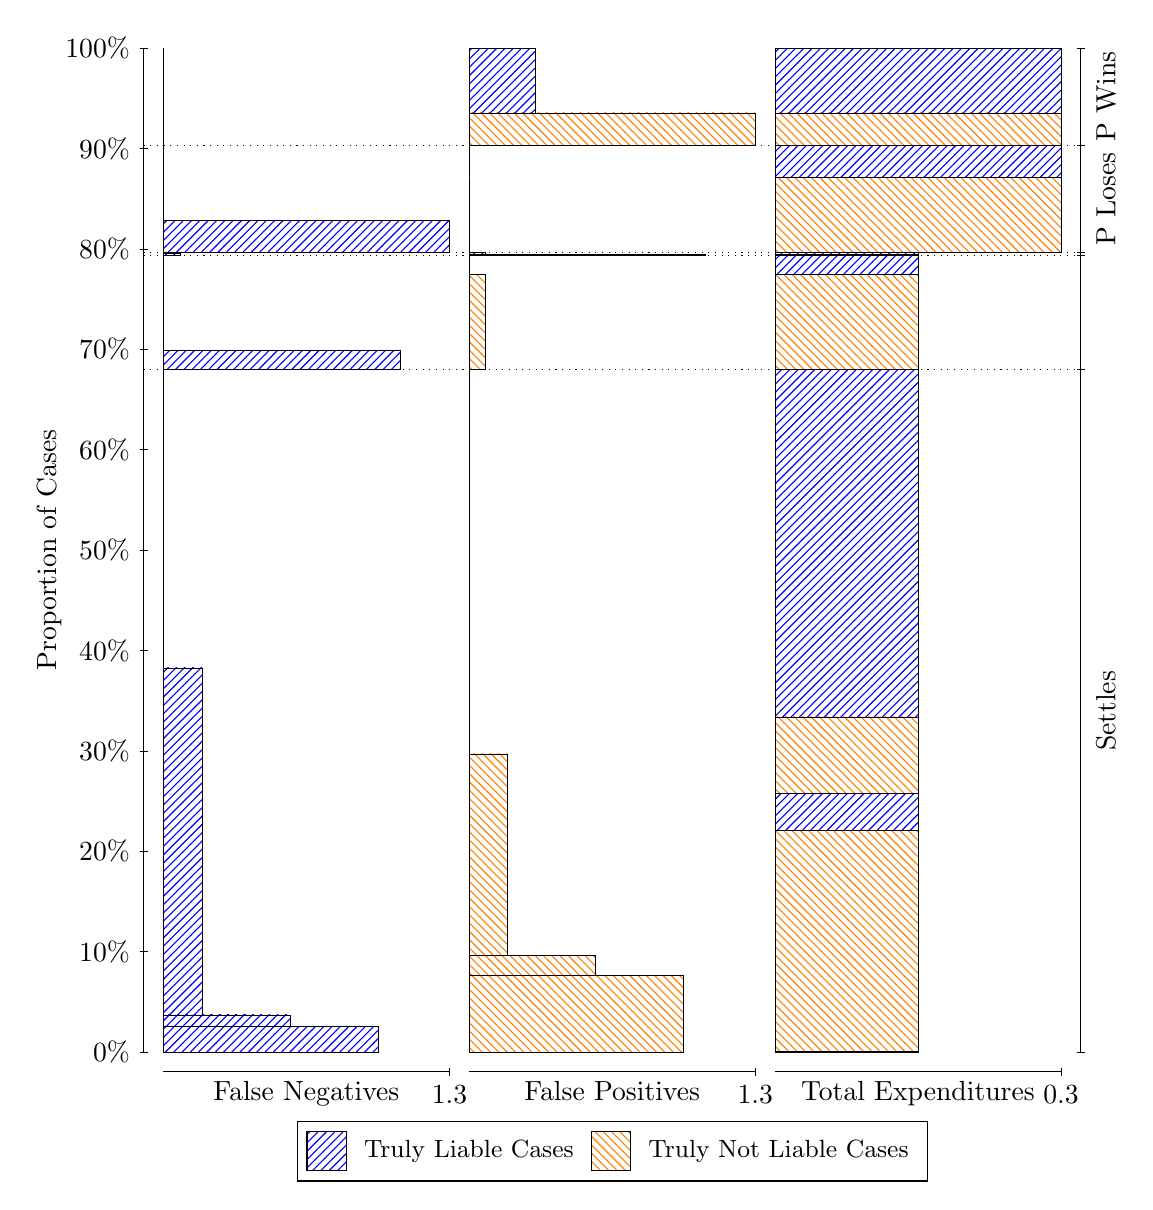
\begin{tikzpicture}
\draw[black, very thin] (1.5,1.75) -- (1.5,14.5);
\node[rotate=90, anchor=center] at (0.3, 8.125) {Proportion of Cases};
\draw[black, very thin] (1.45,1.75) -- (1.55,1.75);
\node[anchor=east] at (1.45, 1.75) {0\%};
\draw[black, very thin] (1.45,3.025) -- (1.55,3.025);
\node[anchor=east] at (1.45, 3.025) {10\%};
\draw[black, very thin] (1.45,4.3) -- (1.55,4.3);
\node[anchor=east] at (1.45, 4.3) {20\%};
\draw[black, very thin] (1.45,5.575) -- (1.55,5.575);
\node[anchor=east] at (1.45, 5.575) {30\%};
\draw[black, very thin] (1.45,6.85) -- (1.55,6.85);
\node[anchor=east] at (1.45, 6.85) {40\%};
\draw[black, very thin] (1.45,8.125) -- (1.55,8.125);
\node[anchor=east] at (1.45, 8.125) {50\%};
\draw[black, very thin] (1.45,9.4) -- (1.55,9.4);
\node[anchor=east] at (1.45, 9.4) {60\%};
\draw[black, very thin] (1.45,10.675) -- (1.55,10.675);
\node[anchor=east] at (1.45, 10.675) {70\%};
\draw[black, very thin] (1.45,11.95) -- (1.55,11.95);
\node[anchor=east] at (1.45, 11.95) {80\%};
\draw[black, very thin] (1.45,13.225) -- (1.55,13.225);
\node[anchor=east] at (1.45, 13.225) {90\%};
\draw[black, very thin] (1.45,14.5) -- (1.55,14.5);
\node[anchor=east] at (1.45, 14.5) {100\%};

\draw[black, very thin] (13.4,1.75) -- (13.4,14.5);
\draw[black, very thin] (13.35,1.75) -- (13.45,1.75);
\node[anchor=west] at (13.35, 1.75) {};
\draw[black, very thin] (13.35,10.414) -- (13.45,10.414);
\node[anchor=west] at (13.35, 10.414) {};
\draw[black, very thin] (13.35,11.869) -- (13.45,11.869);
\node[anchor=west] at (13.35, 11.869) {};
\draw[black, very thin] (13.35,11.9) -- (13.45,11.9);
\node[anchor=west] at (13.35, 11.9) {};
\draw[black, very thin] (13.35,13.266) -- (13.45,13.266);
\node[anchor=west] at (13.35, 13.266) {};
\draw[black, very thin] (13.35,14.5) -- (13.45,14.5);
\node[anchor=west] at (13.35, 14.5) {};

\draw[black, very thin, pattern color=blue, pattern=north east lines] (1.75,1.75) rectangle (4.475,2.074);
\draw[black, very thin, pattern color=blue, pattern=north east lines] (1.75,2.074) rectangle (4.1955,2.0745);
\draw[black, very thin, pattern color=blue, pattern=north east lines] (1.75,2.0745) rectangle (3.916,2.075);
\draw[black, very thin, pattern color=blue, pattern=north east lines] (1.75,2.075) rectangle (3.6365,2.0756);
\draw[black, very thin, pattern color=blue, pattern=north east lines] (1.75,2.0756) rectangle (3.3571,2.2202);
\draw[black, very thin, pattern color=blue, pattern=north east lines] (1.75,2.2202) rectangle (3.0776,2.2207);
\draw[black, very thin, pattern color=blue, pattern=north east lines] (1.75,2.2207) rectangle (2.7981,2.2211);
\draw[black, very thin, pattern color=blue, pattern=north east lines] (1.75,2.2211) rectangle (2.5186,2.2216);
\draw[black, very thin, pattern color=blue, pattern=north east lines] (1.75,2.2216) rectangle (2.2391,6.6287);
\draw[black, very thin, pattern color=orange, pattern=north west lines] (1.75,6.6287) rectangle (1.75,10.414);
\draw[black, very thin, pattern color=blue, pattern=north east lines] (1.75,10.414) rectangle (4.7545,10.657);
\draw[black, very thin, pattern color=orange, pattern=north west lines] (1.75,10.657) rectangle (1.75,11.869);
\draw[black, very thin, pattern color=blue, pattern=north east lines] (1.75,11.869) rectangle (1.9596,11.888);
\draw[black, very thin, pattern color=orange, pattern=north west lines] (1.75,11.888) rectangle (1.75,11.9);
\draw[black, very thin, pattern color=blue, pattern=north east lines] (1.75,11.9) rectangle (5.3833,12.311);
\draw[black, very thin, pattern color=orange, pattern=north west lines] (1.75,12.311) rectangle (1.75,13.266);
\draw[black, very thin, pattern color=orange, pattern=north west lines] (1.75,13.266) rectangle (1.75,13.676);
\draw[black, very thin, pattern color=blue, pattern=north east lines] (1.75,13.676) rectangle (1.75,14.5);
\draw[black, very thin, pattern color=orange, pattern=north west lines] (5.6333,1.75) rectangle (8.3583,2.7199);
\draw[black, very thin, pattern color=orange, pattern=north west lines] (5.6333,2.7199) rectangle (8.0788,2.7213);
\draw[black, very thin, pattern color=orange, pattern=north west lines] (5.6333,2.7213) rectangle (7.7994,2.7226);
\draw[black, very thin, pattern color=orange, pattern=north west lines] (5.6333,2.7226) rectangle (7.5199,2.7239);
\draw[black, very thin, pattern color=orange, pattern=north west lines] (5.6333,2.7239) rectangle (7.2404,2.9718);
\draw[black, very thin, pattern color=orange, pattern=north west lines] (5.6333,2.9718) rectangle (6.9609,2.9719);
\draw[black, very thin, pattern color=orange, pattern=north west lines] (5.6333,2.9719) rectangle (6.9609,2.9737);
\draw[black, very thin, pattern color=orange, pattern=north west lines] (5.6333,2.9737) rectangle (6.6814,2.9756);
\draw[black, very thin, pattern color=orange, pattern=north west lines] (5.6333,2.9756) rectangle (6.4019,2.9774);
\draw[black, very thin, pattern color=orange, pattern=north west lines] (5.6333,2.9774) rectangle (6.1224,5.5353);
\draw[black, very thin, pattern color=blue, pattern=north east lines] (5.6333,5.5353) rectangle (5.6333,10.414);
\draw[black, very thin, pattern color=orange, pattern=north west lines] (5.6333,10.414) rectangle (5.8429,11.626);
\draw[black, very thin, pattern color=blue, pattern=north east lines] (5.6333,11.626) rectangle (5.6333,11.869);
\draw[black, very thin, pattern color=orange, pattern=north west lines] (5.6333,11.869) rectangle (8.6378,11.881);
\draw[black, very thin, pattern color=blue, pattern=north east lines] (5.6333,11.881) rectangle (5.8429,11.9);
\draw[black, very thin, pattern color=orange, pattern=north west lines] (5.6333,11.9) rectangle (5.6333,12.855);
\draw[black, very thin, pattern color=blue, pattern=north east lines] (5.6333,12.855) rectangle (5.6333,13.266);
\draw[black, very thin, pattern color=orange, pattern=north west lines] (5.6333,13.266) rectangle (9.2667,13.676);
\draw[black, very thin, pattern color=blue, pattern=north east lines] (5.6333,13.676) rectangle (6.4718,14.5);
\draw[black, very thin, pattern color=orange, pattern=north west lines] (9.5167,1.75) rectangle (11.333,1.7556);
\draw[black, very thin, pattern color=blue, pattern=north east lines] (9.5167,1.7556) rectangle (11.333,1.7572);
\draw[black, very thin, pattern color=orange, pattern=north west lines] (9.5167,1.7572) rectangle (11.333,4.563);
\draw[black, very thin, pattern color=blue, pattern=north east lines] (9.5167,4.563) rectangle (11.333,5.0316);
\draw[black, very thin, pattern color=orange, pattern=north west lines] (9.5167,5.0316) rectangle (11.333,6.0055);
\draw[black, very thin, pattern color=blue, pattern=north east lines] (9.5167,6.0055) rectangle (11.333,10.414);
\draw[black, very thin, pattern color=orange, pattern=north west lines] (9.5167,10.414) rectangle (11.333,11.626);
\draw[black, very thin, pattern color=blue, pattern=north east lines] (9.5167,11.626) rectangle (11.333,11.869);
\draw[black, very thin, pattern color=orange, pattern=north west lines] (9.5167,11.869) rectangle (11.333,11.881);
\draw[black, very thin, pattern color=blue, pattern=north east lines] (9.5167,11.881) rectangle (11.333,11.9);
\draw[black, very thin, pattern color=orange, pattern=north west lines] (9.5167,11.9) rectangle (13.15,12.855);
\draw[black, very thin, pattern color=blue, pattern=north east lines] (9.5167,12.855) rectangle (13.15,13.266);
\draw[black, very thin, pattern color=orange, pattern=north west lines] (9.5167,13.266) rectangle (13.15,13.676);
\draw[black, very thin, pattern color=blue, pattern=north east lines] (9.5167,13.676) rectangle (13.15,14.5);
\draw[black, dotted] (1.5,10.414) -- (13.4,10.414);
\draw[black, dotted] (1.5,11.869) -- (13.4,11.869);
\draw[black, dotted] (1.5,11.9) -- (13.4,11.9);
\draw[black, dotted] (1.5,13.266) -- (13.4,13.266);
\draw[black, very thin] (1.75,1.5) -- (5.3833,1.5);
\node[anchor=north] at (3.5667, 1.5) {False Negatives};
\draw[black, very thin] (5.3833,1.45) -- (5.3833,1.55);
\node[anchor=north] at (5.3833, 1.45) {1.3};

\draw[black, very thin] (5.6333,1.5) -- (9.2667,1.5);
\node[anchor=north] at (7.45, 1.5) {False Positives};
\draw[black, very thin] (9.2667,1.45) -- (9.2667,1.55);
\node[anchor=north] at (9.2667, 1.45) {1.3};

\draw[black, very thin] (9.5167,1.5) -- (13.15,1.5);
\node[anchor=north] at (11.333, 1.5) {Total Expenditures};
\draw[black, very thin] (13.15,1.45) -- (13.15,1.55);
\node[anchor=north] at (13.15, 1.45) {0.3};

\node[black, centered, rotate=90] at (13.72, 6.082) {Settles};


\node[black, centered, rotate=90] at (13.72, 12.583) {P Loses};
\node[black, centered, rotate=90] at (13.72, 13.883) {P Wins};

\draw (7.449999999999999,1.5) node[draw=none] (baseCoordinate) {};
\begin{scope}[align=center]
        \matrix[scale=0.5, draw=black, below=0.5cm of baseCoordinate, nodes={draw}, column sep=0.1cm]{
            \node[rectangle, draw, minimum width=0.5cm, minimum height=0.5cm, pattern=north east lines, pattern color=blue] {}; &
            \node[draw=none, font=\small] (B) {Truly Liable Cases}; &
            \node[rectangle, draw, minimum width=0.5cm, minimum height=0.5cm, pattern=north west lines, pattern color=orange] {}; &
            \node[draw=none, font=\small] (B) {Truly Not Liable Cases}; \\
            };
\end{scope}

\end{tikzpicture}
\end{document}